\section{lib/Efreet\_\-Mime.h File Reference}
\label{Efreet__Mime_8h}\index{lib/Efreet\_\-Mime.h@{lib/Efreet\_\-Mime.h}}


\subsection{Detailed Description}
The file that must be included by any project wishing to use. 





This graph shows which files directly or indirectly include this file:\nopagebreak
\begin{figure}[H]
\begin{center}
\leavevmode
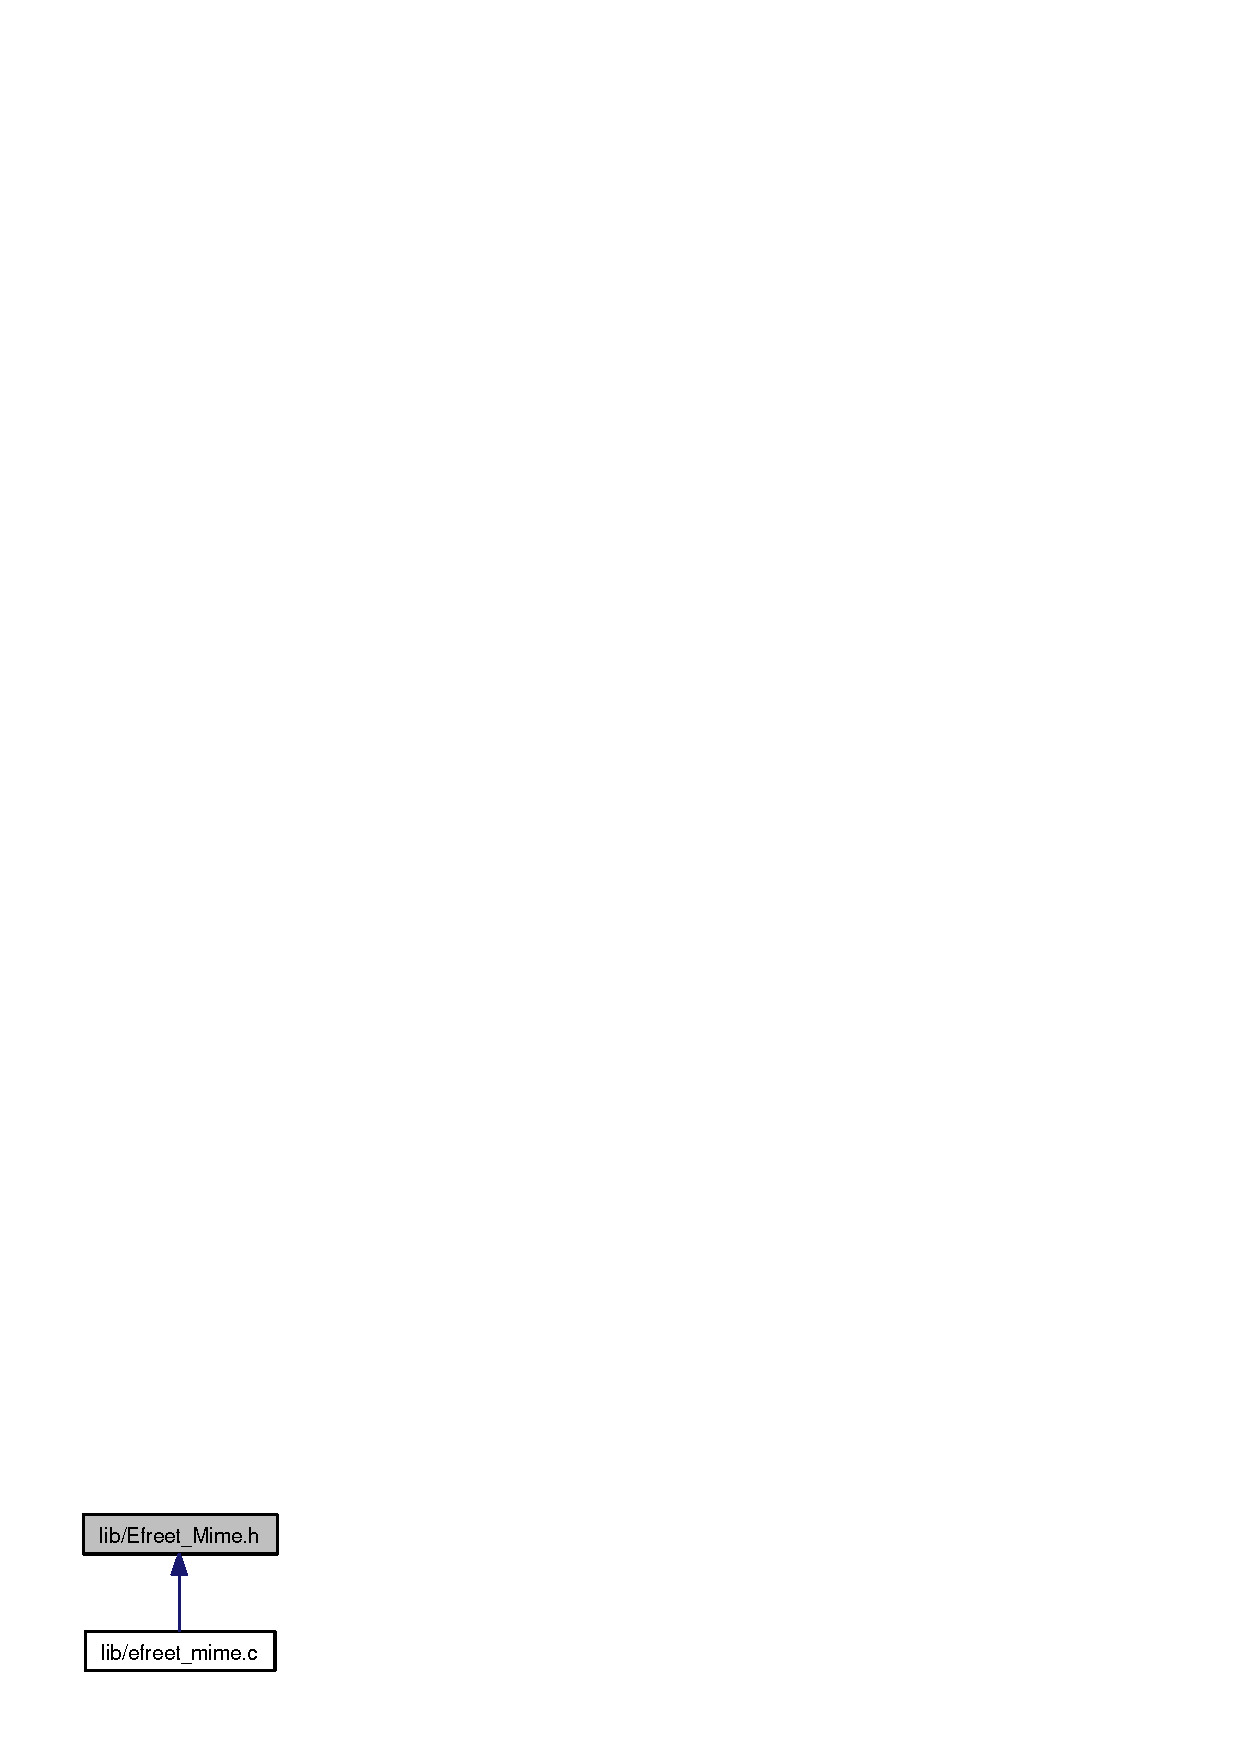
\includegraphics[width=71pt]{Efreet__Mime_8h__dep__incl}
\end{center}
\end{figure}
\subsection*{Defines}
\begin{CompactItemize}
\item 
\#define {\bf EAPI}
\end{CompactItemize}
\subsection*{Functions}
\begin{CompactItemize}
\item 
EAPI const char $\ast$ {\bf efreet\_\-mime\_\-fallback\_\-type\_\-get} (const char $\ast$file)
\begin{CompactList}\small\item\em Retreive the fallback mime type of a file. \item\end{CompactList}\item 
EAPI const char $\ast$ {\bf efreet\_\-mime\_\-globs\_\-type\_\-get} (const char $\ast$file)
\begin{CompactList}\small\item\em Retreive the mime type of a file using globs. \item\end{CompactList}\item 
EAPI int {\bf efreet\_\-mime\_\-init} (void)
\begin{CompactList}\small\item\em Initializes the efreet mime settings. \item\end{CompactList}\item 
EAPI const char $\ast$ {\bf efreet\_\-mime\_\-magic\_\-type\_\-get} (const char $\ast$file)
\begin{CompactList}\small\item\em Retreive the mime type of a file using magic. \item\end{CompactList}\item 
EAPI void {\bf efreet\_\-mime\_\-shutdown} (void)
\begin{CompactList}\small\item\em Cleans up the efreet mime settings system. \item\end{CompactList}\item 
EAPI const char $\ast$ {\bf efreet\_\-mime\_\-special\_\-type\_\-get} (const char $\ast$file)
\begin{CompactList}\small\item\em Retreive the special mime type of a file. \item\end{CompactList}\item 
EAPI const char $\ast$ {\bf efreet\_\-mime\_\-type\_\-get} (const char $\ast$file)
\begin{CompactList}\small\item\em Retreive the mime type of a file. \item\end{CompactList}\item 
EAPI char $\ast$ {\bf efreet\_\-mime\_\-type\_\-icon\_\-get} (const char $\ast$mime, const char $\ast$theme, unsigned int size)
\begin{CompactList}\small\item\em Retreive the mime type icon for a file. \item\end{CompactList}\end{CompactItemize}
